%\documentstyle[epsf,twocolumn]{jarticle}       %LaTeX2.09仕様
%\documentclass[twocolumn]{jarticle}     %pLaTeX2e仕様
\documentclass{jarticle}     %pLaTeX2e仕様

%一枚組だったら[twocolumn]関係のとこ消す

\setlength{\topmargin}{-45pt}
%\setlength{\oddsidemargin}{0cm} 
\setlength{\oddsidemargin}{-7.5mm}
%\setlength{\evensidemargin}{0cm} 
\setlength{\textheight}{24.1cm}
%setlength{\textheight}{25cm} 
\setlength{\textwidth}{17.4cm}
%\setlength{\textwidth}{172mm} 
\setlength{\columnsep}{11mm}

\kanjiskip=.07zw plus.5pt minus.5pt

\usepackage[dvipdfm]{graphicx}
\usepackage{ccaption}
\usepackage{algorithm}
\usepackage{algorithmic}
\usepackage{subcaption}
\usepackage{enumerate}
\usepackage{comment}
\usepackage{url}
\usepackage{multirow}
\usepackage{diagbox}
\usepackage{amssymb}
\usepackage{mathtools}
\usepackage{wrapfig}
\usepackage{graphicx}
\usepackage{float}
\usepackage{amsmath}
\usepackage{lipsum}


\begin{document}
  \noindent
  \hspace{1em}

  \today Creation班 ゼミ
  \hfill
  \ \  西村昭賢 

  \vspace{2mm}
  \hrule
  \begin{center}
  {\Large \bf 進捗報告}
  \end{center}
  \hrule
  \vspace{3mm}


\section{自己対戦の実装}
図 \ref{fig:selfplay} に実装したい自己対戦の形を示す.
また, 図 \ref{fig:initail} に実装した自己対戦において, 先週までは初期のモデルは図 \ref{fig:initail} の上部で作成したモデルを用いていたが強いモデルとなっていなかったため, 対戦相手に定期的にルールベースのモデルを入れて学習を進める形を実装しようとした. \par
対戦相手がルールベースとなった際にゲームが終了しないバグが発生しているので現在その調査をしています.


\begin{figure}[ht]
  \centering
  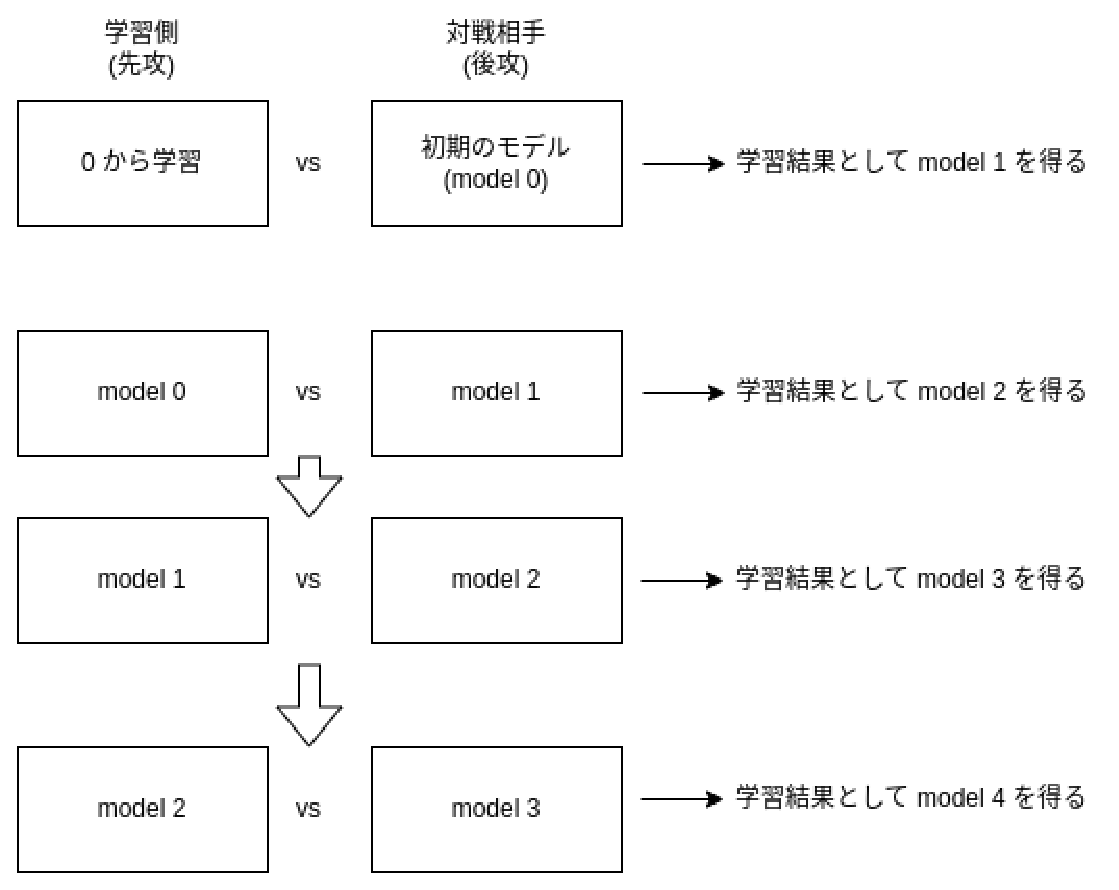
\includegraphics[width=120mm]{assets/modelprogress.eps}
  \vspace{-0.3cm}
  \caption{自己対戦のフロー}
  \label{fig:selfplay}
\end{figure}

\begin{figure}[ht]
  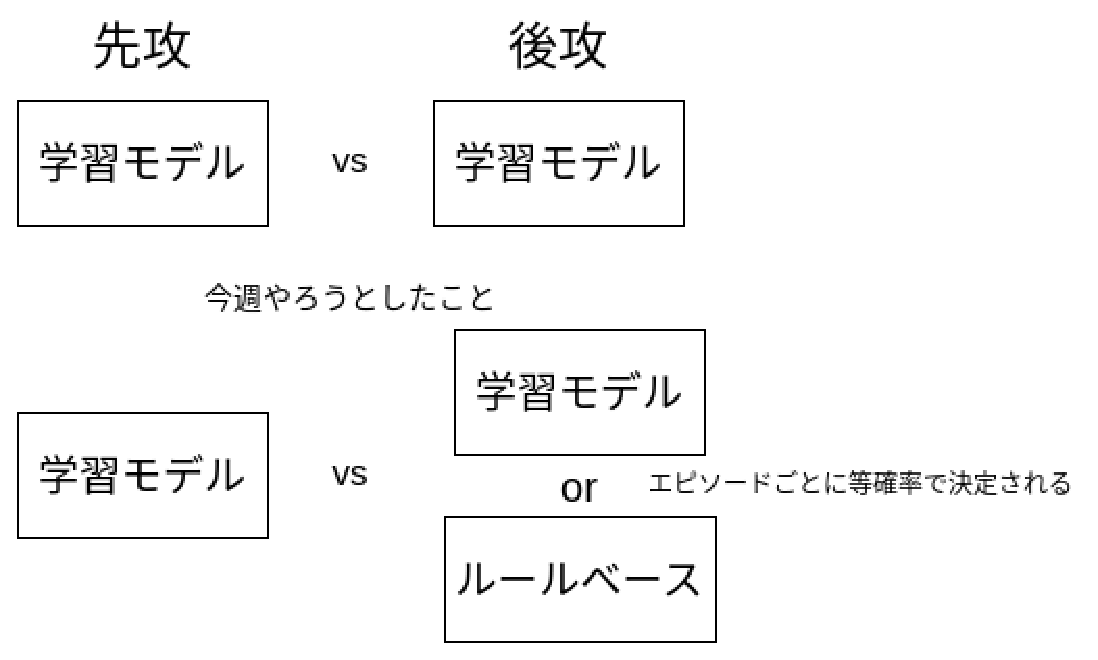
\includegraphics[width=120mm]{assets/Initail.eps}
  \vspace{-0.3cm}
  \caption{初期モデルの訓練}
  \label{fig:initail}
\end{figure}

\section{ChatGPT によるシミュレーションの相談}

図 \ref{fig:flow}に GPT4.0 の ChatGPT にカードプールを生成してもらい役職付き TCG のゲームバランスの調整を行う実験に関して, これからは GPT4 の ChatGPT に生成したもらったカードの実装を進めていく予定ですが, 2 点ほど相談したい点があります.

\begin{figure}[ht]
  \centering
  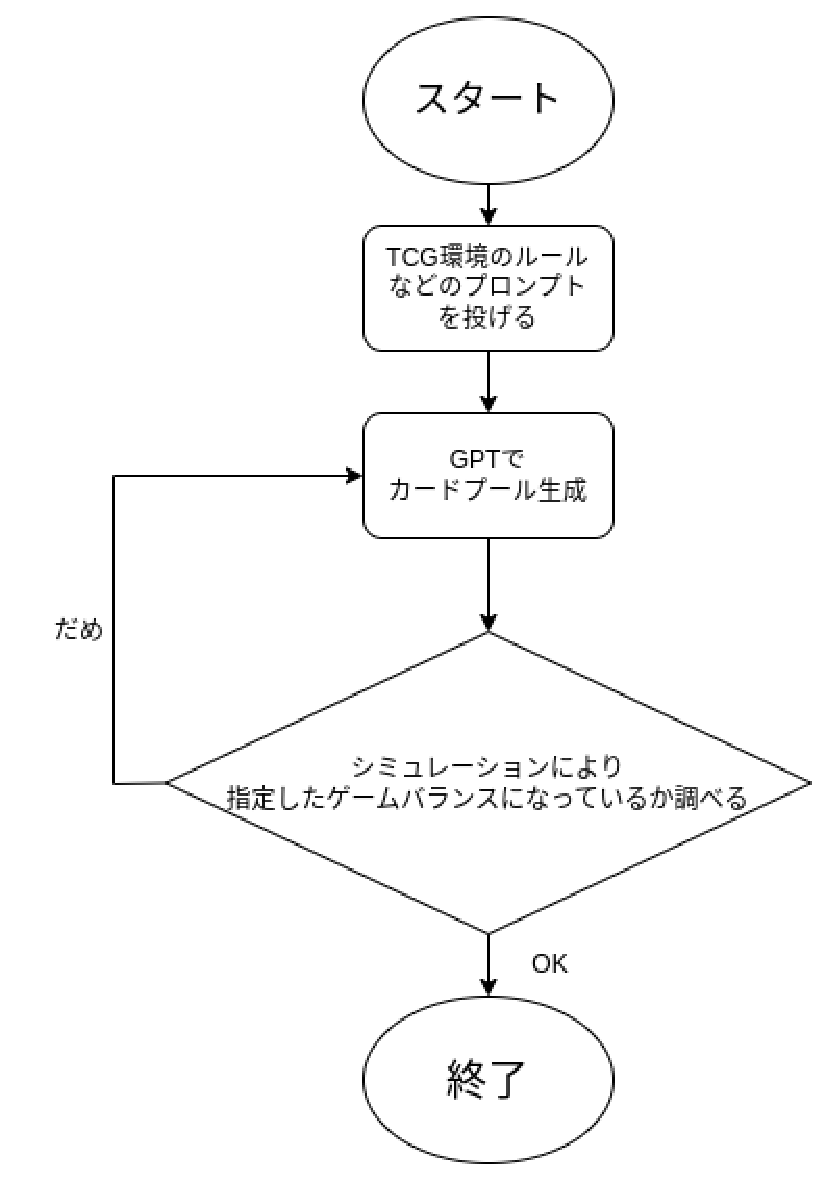
\includegraphics[width=120mm]{assets/flow.eps}
  \vspace{-0.3cm}
  \caption{実験の簡単なフローチャート}
  \label{fig:flow}
\end{figure}

\subsection{役職間のバランス}
図 \ref{fig:deck} に現時点で考えている役職間のバランスを示す. \par
ある程度有利不利の関係は決めたのですが, ChatGPT にプロンプト内でゲームバランスがどのような状況になれば理想的な状況か指定する必要があると考えています. 具体的な勝率の値に関して有利状況の場合は勝率が60 \% くらいに考えています. この勝率が妥当なものか相談したいです.

\subsection{シミュレーションについて}
どのように強化学習を絡めていけばよいか相談したいです.

\begin{figure}[ht]
  \centering
  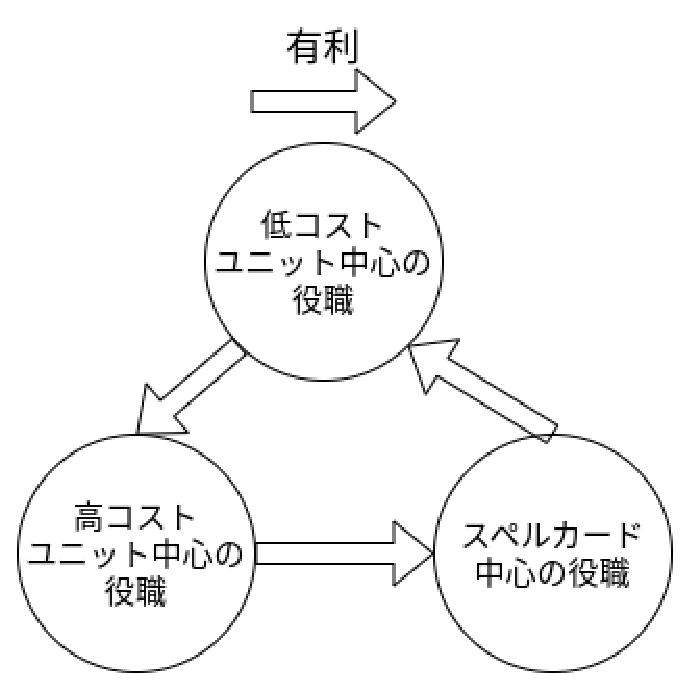
\includegraphics[width=120mm]{assets/deck.eps}
  \vspace{-0.3cm}
  \caption{役職間のバランス案}
  \label{fig:deck}
\end{figure}


%index.bibはtexファイルと同階層に置く
%ちゃんと\citeしないと表示されない(1敗)
\bibliography{index.bib}
\bibliographystyle{junsrt}

\end{document}